  % !TEX TS?program = pdflatexmk
                    \documentclass[a4paper, 12pt]{article}
                  \usepackage[english]{babel}
                  \usepackage[utf8]{inputenc}
    		\usepackage[utf8]{inputenc}
    %                \renewcommand{\baselinestretch}{1.0} 
                    
                    
                    %MARGINS
                    \usepackage[left=25.4mm, right = 25.4mm, top=25.4mm, bottom=25.4mm, includefoot]{geometry}
      %            \geometry{a4paper, total={170mm,257mm}, left=25.4mm, right = 25.4mm, top=25.4mm, bottom=25.4mm}
                    \setlength{\parindent}{0in}
                    \usepackage{enumitem}
                   
                    %Adding pictures
                    \usepackage{graphicx}
                    \usepackage{float}
                    
                    %Header and footers
                    \usepackage{fancyhdr}
                    \pagestyle{fancy}
%                    \fancyhead{}
                    \fancyfoot{}
                    \fancyfoot[R]{ \thepage\ }
                    \renewcommand{\headrulewidth}{0pt} %change the pt width to insert header line
                    \renewcommand{\footrulewidth}{0pt} %change the pt width to insert footer line
                    \usepackage{amsmath}
                    \fancyhf{}
                    
%    	\rhead{\leftmark}
%    	\lhead{Guides and tutorials}
	\rfoot{Centre for Civil Society \hspace{1mm} \textbar \hspace{1mm} www.ccs.in \hspace{2mm}  \thepage}
%             \lfoot{  \leftmark }     			% get the section heading on the footer 
                   
                   
                    %Tables
                    \usepackage{booktabs}
                    \usepackage{subfig}
                    \captionsetup{aboveskip=14pt,}
                    \captionsetup[table]{singlelinecheck = false}
                     \newcommand\tabitem{\makebox[1em][r]{\textbullet~}}
                     \usepackage{longtable}
                    
                    %Coloured Boxes
                    \usepackage{xcolor}
                    \usepackage{mdframed}
                    
                    %Custom Spacing
                    \usepackage{setspace}
                    
                    %Defining Colours
             \definecolor{CCSbrown}{RGB}{163, 86, 37}
               \definecolor{CCSgrey}{RGB}{105, 105, 105}
                 \definecolor{CCSblack}{RGB}{64, 64, 65} 
             
             
             %Heading colours                  
                    \usepackage{sectsty}
                    \usepackage{titlesec}
    		\chapterfont{\color{blue}}  % sets colour of chapters font
    		\sectionfont{\color{CCSbrown}}  %sets colour of section font
    		\subsectionfont{\color{CCSblack}} %sets colour of subsection font
    		\subsubsectionfont{\color{CCSgrey}} %sets colour of subsubsection font
    		
		
		%Bibliography
		
		\usepackage[authordate, backend=biber]{biblatex-chicago}
		\addbibresource{CRA.bib}
		\usepackage{hyperref} %[hidelinks]?
		\hypersetup{
		colorlinks,
		linkcolor = black,
		citecolor = blue}
		\usepackage{blindtext}
		
              %Tables 
              \usepackage{array}
              \usepackage{makecell}
              \usepackage{tabularx}	
              \newcolumntype{$}{>{\global\let\currentrowstyle\relax}}
              \newcolumntype{^}{>{\currentrowstyle}}
              \newcommand{\rowstyle}[1]{\gdef\currentrowstyle{#1}#1\ignorespaces}
             
\begin{document}
                    
    %==================================================                
                    %TITLE PAGE
                    \begin{titlepage}
                    	\begin{center}
                    	\line(1,0){300}\\
                    	[0.25in]
                    	\huge{\bfseries \textcolor{CCSbrown} {Risky Business}} \\
    	[0.5cm]
    	\large  {Assessing the Pollution Monitoring and Enforcement Framework\\  for Enterprises in Delhi} \\
    	
                    	\line(1,0){200}\\
                    	[1in]
                    	\textsc{\huge Ayesha Selwyn, \\ Parth Singh, Pushyami Chilakapati} \\
                    	[1.5cm]
                    	{\Large September 2018} \\
                    	[2.0cm]
    %    	{\huge Researching Reality Internship 2018} \\
     %   	[0.5cm]
                    	{\LARGE Centre for Civil Society} \\
                    	[0.1mm]
                    	{\Large New Delhi, India} \\
    	[2.0cm]
    	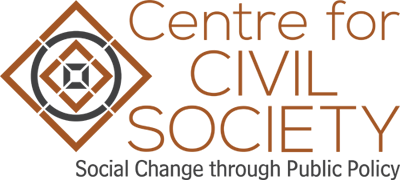
\includegraphics[width = 75mm]{unnamed.png}
      
                    	\end{center}
                    \end{titlepage}
                     %=====================TOC===============================================                 
                    \tableofcontents
                    
     %======================LIST OF ABBREVIATIONS================================         
                   \newpage
                   \newlist{abbrv}{itemize}{1}
        \setlist[abbrv,1]{label=,labelwidth=1in,align=parleft,itemsep=0.1\baselineskip,leftmargin=!}
         
        \section*{List of Abbreviations}
        \addcontentsline{toc}{section}{List of Abbreviations}
        %\chaptermark{List of Abbreviations}
       
        
        \begin{abbrv}
        \item[BRAP]			Business Reforms Action Plan
        \item[CPCB]			Central Pollution Control Board
        \item[CRA]			Computerised Risk Assessment
        \item[CTE]				Consent to Establish
        \item[CTO]			Consent to Operate
        \item[DIPP]			Department of Industrial Policy and Promotion
        \item[DPCC]			Delhi Pollution Control Committee
        \item[DG]				Diesel Generator
        \item[EE]				Environmental Engineer
        \item[SEE]		                 Senior Environmental Engineer
        \item[SOP]			Standard Operating Procedure
        \item[SPCB]			State Pollution Control Board
        \item[VPI]				Visit Priority Index 
          
        
         
        \end{abbrv}
        
                    
                    %EXECUTIVE SUMMARY
                    \newpage
                    \section*{Executive Summary}
                    \addcontentsline{toc}{section}{Executive Summary}
                    The 2017 Business Reform Action Plan (BRAP) of the Department of Industrial Policy and Promotion (DIPP) of the Ministry of Commerce and Industry presented 405 recommendations for states to implement for improving the business climate, including six reforms to the way regulatory inspections are carried out. \\
                  
                  A rationalised, consistent and effective inspection regime is the starting point for regulatory enforcement. Unfortunately, inspections have long been infamous in India as the breeding ground for corruption and the extortion of money by government officials based on discretionary powers assigned to them \parencite{PHD}. With the focus on ease of doing business, reforms to end the inspector raj \parencite{livemint}(Nanda 2014) have been front and centre on the agenda. \\
                  
                  The six inspection enabler reforms suggested by the DIPP can potentially change the way inspections are conducted today, particularly in the area of environmental compliance by the State Pollution Control Boards (SPCB). A risk-based approach to target inspections, transparency measures and process checklists, introduced in this round of reforms, are some of the best practices implemented globally for inspection reform (Blanc 2012, p. 3). By introducing a computerised risk assessment system, the SPCBs could reduce the discretionary power Environmental Engineers (EEs) (loosely called inspectors) wield over enterprises. EEs are now required to upload the inspection reports within 48 hours of the inspection, and reports can no longer be modified after they have been uploaded. \\
                  
                 The Delhi Pollution Control Committee (DPCC) is the SPCB responsible for the enforcement of environmental standards for industries in Delhi stipulated under the Air and Water Acts and Hazardous Waste Management Rules \parencite{DPCCb}(Delhi Pollution Control Committee 2016b). \\
                 
                 In this paper, we assess the quality of implementation of different inspection reforms implemented by the DPCC in 2017 as part of the effort to improve the ease of doing business in Delhi. The inspections norms of DPCC have been the primary vehicle through which it ensures compliance and are also how businesses experience regulations and interact with the agency (DPCC 2016b). \\
                 
                 To study the extent to which the DPCC, which is the SPCB of Delhi, has implemented these reform suggestions and assess how the reforms have affected the functioning of DPCC, we interviewed Senior Environmental Engineers (SEEs) and businesses. In the course of our investigation, we also studied the Standard Operating Procedure (SOP) that EEs are required to follow to ensure the consistent implementation of regulations. We have not analysed the content and quality of SOPs or the BRAP reforms and have restricted ourselves to studying the implementation of the SOPs and recommended reforms. \\
                 
                 We find that while the DPCC has implemented some of the reforms it has claimed to, some are executed only partially, failing to meet the intended objectives. For example, the DPCC has published the inspection checklist on its website and now provides a unique login identification (ID) to enterprises to access the inspection reports. However, the DPCC does not yet use risk assessment software to identify enterprises for inspection—a key reform that it has claimed to have implemented. Even now, a committee manually identifies enterprises that are to be inspected. The DPCC claims that it cannot implement this system due to a shortage of personnel, as only 60\% of its sanctioned posts are currently filled. This is counterintuitive, as technology should ease some of the administrative workloads and help officials focus on primary tasks such as site inspection. \\
                 
                 Additionally, we find that EEs only partially follow the SOPs, raising concerns of procedural consistency across inspections. Enterprises are not always asked to sign the inspection report, and a formal notice detailing corrective measures is not always sent to enterprises. Not all enterprises have access to their inspection reports within 24 hours, and not all enterprises are notified of their risk category. Regardless of how well an SOP is designed, if it is not followed, it is likely to fail its intended purpose. \\
                 
                  The DIPP has so far primarily relied on self-reported evidence by states. In 2017, it introduced a system to include business feedback. Although business feedback is key to reform, it has its shortcomings. For instance, a business survey may not be able to judge the efficacy of changes to the back-office functioning of a government department. The current state of affairs calls for a close evaluation of the implementation of reforms, as reliance on self-reported evidence by state governments or a survey of business enterprises may paint a false picture. \\
                  
                  %INTRODUCTION
                    \newpage
                    \section{Introduction}
                    
                 The DPCC enforces national pollution standards in Delhi and is responsible for the ‘entire environmental status of the State’ (National Green Tribunal 2017). \\
                 
                 Although there are over 200 regulations governing environmental protection, the Water (Prevention and Control of Pollution) Act, 1974,\footnote{Last amended in 2003.} and the Air (Prevention and Control of Pollution) Act of 1981\footnote{Amended in 1987.} are the two essential acts that empower SPCBs to regulate the emissions and effluents discharged by any industry (OECD 2006). The DPCC also grants Consent to Establish (CTE) and Consent to Operate (CTO) to industries to establish and operate under these two acts. \\
                 
                 The quality of a regulatory regime and its effectiveness in achieving the regulatory goals depends as much on the way regulations are implemented and enforced as on the design of regulations. Unfortunately, the enforcement and implementation of regulations are not evaluated as often as regulation design, creating an informational lacuna (OECD 2014). \\
                 
                 One of the critical ways of carrying out regulatory action is through inspections. While the regulatory regime sets the rules for compliance, inspectors—who are at the frontlines of enforcement—generally have some autonomy and discretion in the way they enforce regulations (May and Wood 2003, p. 117). For most businesses, inspections are the primary form through which regulations are experienced and are a particularly important concern because they are recurring in nature (Blanc 2012, p. 7). \\
                 
                 Inspection is the primary tool used by the DPCC to monitor and enforce compliance environment standards. As per the Office Order of DPCC dated 26 July 2016, it conducts inspections to meet three objectives: first, to assess pollution potential; second, to evaluate compliance with standards stipulated for industries under the environment acts; and third, to guide industries to improve (DPCC 2016b). \\
                 
                 \subsection{Regulatory Reforms Introduced in 2017}
                 
                 Regulatory reforms are generally motivated by the need to ease the regulatory burden on businesses, to improve compliance and to improve government efficiency. The DIPP, of the Ministry of Commerce and Industry, conceived the BRAP in 2014, primarily to improve the ease of doing business and improve government efficiency. The implementation of reforms is evaluated by the DIPP and the World Bank periodically based on self-reported evidence. As of June 2018, Delhi had implemented 33.9\% of the reforms recommended under the BRAP and was ranked 23rd out of 36 states. \\
                 
                 Besides self-reported evidence, the DIPP and the World Bank also verified implementation through business surveys in 2017. However, there are two challenges in the use of a business survey to evaluate implementation. First, businesses may not be aware of governance changes introduced within government departments, and second, it sought to verify only selected reforms. Some improvements that have no direct bearing on business activity may remain unverified. \\
                 
                 Realising the gaps in evaluating the status of reforms in Delhi, we set out to study the enforcement of one part of the 2017 plan: inspections reforms. These inspections reforms apply to state government departments, such as the Labour Department, SPCBs and the Forest Department. In our study, we have only explored the reforms suggested and implemented by the SPCB in Delhi, that is, the DPCC. \\
                 
                 To streamline the inspection process of the SPCBs, BRAP 2017 recommended six reforms each under the Air and Water Acts. The six reforms under the Air Act are identical to those under the Water Act. \\
                 
                 The six distinct reforms (which are the same for the Air Act and the Water Act) include: \\
                 
                 \begin{enumerate}
                 \item Design and implement a system for identifying enterprises that need to be inspected based on a computerised risk assessment \textit{(Recommendations 165 and 171)}.
                 \item Publish a well-defined inspection procedure and checklist on the department’s website \textit{(Recommendations 164 and 170)}.
                 \item Allow enterprises to view and download submitted inspection reports for at least the past 2 years \textit{(Recommendations 167 and 173)}.
                 \item Mandate the online submission of inspection reports within 48 hours of the inspection to the DPCC \textit{(Recommendations 166 and 172)}.
                 \item Design and implement a system for the computerised allocation of inspectors \textit{(Recommendations 168 and 173)}.
                 \item Mandate that the same inspector will not inspect the same enterprise twice consecutively \textit{(Recommendations 169 and 175)} (Department of Industrial Policy and Promotion 2017a).
                 \end{enumerate}
                 
                 Delhi has provided evidence on the DIPP website on the implementation of a total of three of these six reforms under each Act.\footnote{Recommendations 164, 170, 165, 171, 167, 173.} \\
                 
                 The first reform, identification of enterprises for inspection through a computerised risk assessment (CRA) system, reduces not only the burden of administration (DIPP 2017d) but also the scope for bias in the selection of enterprises and, therefore, the scope for inspector raj (Nanda 2014). \\
                 
                 Computerisation has a couple of benefits: the integration of inspection processes into one system and the elimination of overlapping inspections and the repetition of work (PWC 2017). Findings made by an inspectorate can also be relevant to other agencies. This data can be used to have a current assessment of the risk level of each business, without spending additional resources (OECD, 2014). The identification of enterprises for inspection through a computerised system allows for reduced bias, limits human errors and increases transparency. \\
                 
                 Besides the CRA system, three reforms aim to make information on the inspection procedure publicly available and enable enterprises to view inspection reports online, enhancing transparency.\footnote{Recommendations 164, 170, 167, 173, 166, 172.} Publicly available checklists allow enterprises to be aware of the expectations of them and bring consistency in the enforcement of norms (Blanc 2012, p. 79). Improving access to information is critical to the quality of government service, empowers citizens and ensures greater accountability from government officials. In fact, easy access to regulatory information is associated with improved governance and reduced corruption (Geginat and Saltane 2016, p. 2). \\
                 
                 The paper focuses on the pollution inspection reforms implemented by the DPCC under BRAP 2017. The \hyperref[sec:1]{first section} of the paper examines the implementation status of the CRA system in Delhi, as it is the most substantive recommendation made by the DIPP. The \hyperref[sec:2]{second section} of the paper examines the implementation of other process improvement reforms and presents a preliminary assessment of the use of SOPs for inspection in the DPCC. Study findings are based on structured interviews with government officials at the DIPP, SEEs at the DPCC and enterprises.\footnote{Details of the interviews conducted are in Appendix 1.} \\ %hyperref purpose? shouldn't it include [hidelinks] in the preamble?
                 
                 \section{Assessing the Implementation Status of Computerised Risk Assessment for Environment Inspections}\label{sec:1} 
                 
                 The DIPP recommended that the DPCC should design and implement a computerised system to identify enterprises for inspection based on a risk assessment. Risk is the probability and scale of the impact of an occurrence. Risk assessment has two aspects: identifying risk and taking measures to control or eliminate it (Stoneburner, Goguen and Feringa 2002). In the context of environmental protection, risk assessment refers to evaluating potential harm to humans, flora and fauna (Environmental Protection Agency, n.d.). The assessment of potential harm helps to identify the people and regions most susceptible to the risk, to prioritise hazards\footnote{A hazard is a potential source of harm. It is different from risk, as risk is the probability of the hazard occurring (Hazard and Safety Authority).} and to determine whether control measures are required for a particular hazard. \\
                 
                 Most countries have developed their own method of assessing environmental risk. The DIPP in the BRAP reforms (Recommendations 165 and 171) prescribed the implementation of the CRA system to identify enterprises for inspection. \\ %should recs be italicised to maintain consistency?
                 
                 According to DIPP officials, the CRA system involves using a computer software to assess risk. The results of the CRA system can be used to identify enterprises eligible for inspection. The DIPP recommends that this system of identifying enterprises must be computerised. The computerisation of the risk assessment process reduces the EEs’ role in assigning risk categories to enterprises when they apply for CTE and CTO and in deciding if, when and by whom they have to be inspected. It results in two benefits: elimination of human errors and bias (and scope for rent seeking) during  risk assessment and freeing up the risk assessor’s time. Moreover, computerisation allows for easy and transparent access to the results of assessment and inspection. \\
                 
                 In Sections 3.1. to 3.3., we evaluate the degree to which the computerisation of risk assessment has been introduced. Section 3.1. describes the risk assessment process currently in place, and section 3.2. discusses how the DPCC currently identifies enterprises for inspection post the risk assessment. Section 3.3. examines risk assessment practices in other states. \\ %how to label 3.1 and 3.2?
                 
                 \subsection{Risk Assessment Currently Practised by the Delhi Pollution Control Committee}
                 
                 The DPCC uses the risk assessment method devised by the Central Pollution Control Board (CPCB) in 2016 to assess the risk of industries. It categorises industries as Red, Orange, Green or White based on their potential to pollute air and water. \\
                 
                 The pollution potential index takes into account the emissions of an enterprise (air pollutants), effluents (water pollutants), hazardous waste generated and consumption of resources. The pollution potential index is calculated based on the number and quantity of pollutants typically released by each industry. The current system assumes that each enterprise within an industry type would discharge similar amounts of effluents, emissions and waste and consume similar types and quantities of resources. The score for any industry ranges from 0 to 100, where a higher score indicates a higher pollution potential. \\
                 
                 %TABLE 1


%\begin{tabular}{p{2cm}p{2cm}p{4cm}p{6cm}}

\begin{longtable}{p{2cm}>{\raggedright}p{3.5cm}>{\raggedright}p{3.5cm}>{\raggedright\arraybackslash}p{6cm}}
\caption{CPCB Risk Categories} \\
Risk Category & Pollution Index Score & Validity Period of CTE/CTO & Examples of Activities \\
\midrule
\endfirsthead
Risk Category & Pollution Index Score & Validity Period of CTE/CTO & Examples of Activities \\
\midrule
\endhead
\endfoot
\endlastfoot

Red & 60-100 & 5 years & \tabitem Healthcare establishments. \\
 &  &  &   \tabitem Automobile manufacturing \\
  &  &  &  \tabitem Slaughterhouses \\
Orange & 41-59 & 10 years &  \tabitem Bakery and confectionary units with a production capacity of more than 1 tonne per day with an oven or furnace  \\
 &  &  & \tabitem Hotels with less than t stars or more than 20, but less than 100 beds \\
 &  &  & \tabitem Food and food processing, including fruit and vegetable processing.  \\
Green & 21-40 & 15 years & \tabitem Bakery and confectionary units with a production capacity of less than 1 tonne per day with a gas or electric oven \\
 &  &  &  \tabitem Hotels up to 20 rooms and without boilers \\
 &  &  & \tabitem Digital printing on polyvinyl chloride clothes \\
White & 0-20 & CTE/CTO not required\footnote{White category industries are required to submit undertakings but do not require CTE or CTO.} & \tabitem Repairing electric motors and generators using a dry mechanical process \\
 &  &  & \tabitem Blending and packing of tea \\
 &  &  & \tabitem Packing of powdered milk \\

\end{longtable}

                                  
                 In addition to the risk categories assigned by the CPCB, DPCC uses another set of risk categories for industries—I, II(a) and II(b)—to determine the members of the committee that will issue CTE/CTO to each industry.\\
                 
        %TABLE 2

\begin{longtable}{>{\raggedright}p{2cm}>{\raggedright}p{4cm}>{\raggedright}p{4cm}>{\raggedright\arraybackslash}p{4cm}}
\caption{DPCC Risk Categories} \\
Risk Category & Requirement of Pollution Control Devices & Members of the Committee That Issue CTE/ CTO & DecisionMaking Time Period \\
\midrule
\endfirsthead
Risk Category & Requirement of Pollution Control Devices & Members of the Committee That Issue CTE/ CTO & DecisionMaking Time Period \\
\midrule
\endhead
\endfoot
\endlastfoot

I & Does not require the installation of pollution control devices & SEEs of the concerned cell\footnote{According to the organisational structure available on the DPCC website, there are 11 cells at the DPCC: Planning and Coordination, Cess Assessment, Consent Management, Waste Management, Planning, IT, Enquiry Counter, Environmental Impact Assessment, Laboratory, Legal, Admin and Accounts Cell.} & Decision to issue CTE/CTO to be made within 7 days of receipt of the application \\
 & & &  \\
II(a) & Requires the installation of pollution control devices, such as the sewage or water treatment plants of Delhi Jal Board, common effluent treatment plants, power plants or municipal solid waste plants & \tabitem Chairman  \tabitem Member Secretary \\  \tabitem Two Engineering Professors \\ \tabitem Director, Department of Environment \\ \tabitem SEEs of the concerned cell \\ \tabitem EEs of the concerned cell 
 & Decision to issue CTE/CTO to be made within 30 days of receipt of the application \\
  & & & \\
II(b) & Requires the installation of pollution control devices not listed under category II(a) & \tabitem Member Secretary \\ \tabitem SEEs of concerned cell \\ \tabitem  EEs of concerned cell & Decision to issue CTE/CTO to be made within 30 days of receipt of the application \\

\end{longtable}
         
                 
                 The system to assign industries a CPCB risk category (Red, Orange, Green or White) and a DPCC risk category [I, II(a) or II(b)] has been computerised.\footnote{This computerised system was designed by M/s Srijan Webmatics.} When an enterprise applies online for CTE or CTO from the DPCC, it is automatically assigned both risk categories based on its type of activity.\footnote{Before this system was in place, if an enterprise wanted to know its risk category, it had to refer to the list of CPCB risk categories (Red, Orange, Green or White) available on the DPCC website.} Consents were earlier issued through a manual system and now are being issued via a computer interface based on the manual system. This essentially means that the manual system has merely been digitised but the basis for determining risk has not been computerised. \\

	\subsection{Current System of Identifying Enterprises Using Computerised Risk Assessment}
	
	\textbf{While the DPCC has claimed to implement a computerised system to identify enterprises for inspection} (DIPP 2017b)\textbf{, in practice, the function is still carried out manually.} \\
	
	According to the DPCC Office Order dated 26 July 2016, the computerised system, if implemented by the DPCC, is supposed to apply the following frequency to inspections: \\
	
	\begin{itemize}
	\item{Enterprises in category II(a) to be inspected before CTE/CTO/Renewal is issued;}
	\item{Monthly inspections of 5\% of enterprises from category II(a) that have been issued CTO;}
	\item{Monthly inspections of 4\% of enterprises from category II(b) that have been issued CTO;}
	\item{Monthly inspections of 1\% of enterprises from category I that have been issued CTO (DPCC 2016b).}
	\end{itemize} 
	
	However, such a system does not exist. The DPCC SEEs we interviewed argued that a shortage of workforce in the department is the reason for the absence of a fixed schedule. An official from the DPCC confirmed that out of 267 sanctioned positions, 105 positions are currently vacant. The SEEs claimed that no new recruitments have been made since 1993 and that there were only 30 engineers in the department. According to the SEEs, a computerised system to identify and schedule inspections would not yield any benefit, as they do not have enough EEs in the department to conduct the number of inspections that a computerised identification system would schedule. \\
	
	Currently, inspections are only conducted for three types of enterprises: (1) Those for whom a court order mandates inspection, (2) Those that have a complaint against them and (3) Those that have applied for CTE/CTO. The Executive Committee identifies the latter two. The Executive Committee does not have a fixed schedule, but they meet once a month on an average, according to the SEE. This means that enterprises are not inspected at random based on their risk category, as they are supposed to be, and there are no regular checks on enterprises, raising concerns over the implementation of environmental standards in Delhi. \\
	
	\subsection{Risk Assessment Practices in Other States}
	
	As of June 2017, 20 SPCBs (including Delhi) have claimed to implement a CRA system.\footnote{Andhra Pradesh, Assam, Bihar, Chhattisgarh, Delhi, Goa, Gujarat, Haryana, Himachal Pradesh, Jharkhand, Karnataka, Madhya Pradesh, Maharashtra, Odisha, Rajasthan, Tamil Nadu, Telangana, Uttarakhand, Uttar Pradesh and West Bengal.} The computerised system in most state relies primarily on the risk category defined by the CPCB. The CPCB risk categorisation assumes that each enterprise within an industry type discharges similar amounts of effluents, emissions and waste and consumes similar types and quantities of resources. It does not depend on the actual amount of emissions or effluents discharged by each enterprise. \\
	
	However, some states have employed additional measures in the risk assessment process, such as the Green category exemption, mandated timeline and size of the industry.\footnote{We have not verified the implementation status of the risk assessment processes in these states. The information here is based on claims made by the states on the DIPP website corresponding to Recommendations 165 and 171 (design and implement a system to identify enterprises to be inspected based on the CRA system).} \\
	
	Three states have \textbf{exempted inspection post-CTE for industries in the Green category} (DIPP 2017d).\footnote{West Bengal, Telangana and Karnataka.} Such enterprises are only inspected in case of any complaints issued or court orders mandating inspection. This is in contrast to the CPCB norm, wherein only White category industries are exempted from obtaining CTE/CTO from SPCBs. While the DPCC currently conducts inspections based only on complaints, court orders or CTE/CTO/Renewal applications, it does not officially exempt Green category enterprises from being inspected. \\
	
	Fifteen states have introduced a \textbf{mandated timeline} for compliance inspections.\footnote{Andhra Pradesh, Assam, Bihar, Chhattisgarh, Gujarat, Haryana, Himachal Pradesh, Jharkhand, Maharashtra, Odisha, Rajasthan, Tamil Nadu, Telangana, Uttarakhand and West Bengal.} The SPCBs in each of these states have prescribed the frequency of inspections for enterprises in each risk category. This frequency also takes into consideration the size and pollution potential of a particular industry. Based on this frequency, they have fixed a schedule for inspections. For example, in Himachal Pradesh, an industry which falls under the Red category and is categorised as a large industry has to be inspected fortnightly while a small-sized Green industry has to be inspected annually (Himachal Pradesh Pollution Control Board 2017). Delhi does not take into consideration the size of the industries and there is no fixed schedule of inspections. \\
	
	Some states use parameters beyond those prescribed by the CPCB such as the \textbf{size of the industry} (calculated on the basis of the type of machinery installed and the area of the industrial unit), \textbf{capital invested} and \textbf{time elapsed since the inspection was due} (as per the mandated timeline for each industry). The score on these parameters is added to the overall risk score to prioritise large industries or those whose inspection has been long due compared to the ones inspected on time as per the mandated timeline. \\
	
	The Gujarat Pollution Control Board has developed a single integrated software called the Xtended Green Node (Gujarat Pollution Control Board 2015). The \textbf{Xtended Green Node} is an integrated software that performs the live monitoring of air and water quality, handles online consent management of CTE/CTO, performs the risk-based identification of industries and randomly allocates inspectors. The software has been replicated in five other states.\footnote{Goa, Himachal Pradesh, Karnataka, Madhya Pradesh and Uttarakhand.} \\
	
	As per the evidence provided on the DIPP portal, SPCBs in Gujarat (Gujarat Pollution Control Board 2015) and Uttarakhand (Uttarakhand Environment Protection and Pollution Control Board 2017) have further designed a Visit Priority Index (VPI) which supplements the existing risk assessment parameters to identify and inspect enterprises. The VPI is calculated as follows: $$VPI = R_c *F_c$$ where $R_c$ is the risk category and $F_c$ is the frequency criteria. \\
	
	$R_c = A*B$, where \\
	
	A is the factor based on pollution potential; \\
	
	B is the factor based on the size of the industry/installation. \\
	
	$F_c = C*D$, where \\
	
	C is the factor based on the frequency of visits to the industrial unit; \\
	
	D is the factor for any exemption from inspections granted to units. \\
	
	While the DPCC does have a CRA system in place, other states use more parameters to measure risk than the DPCC does. These additional parameters aim to reduce human interference in the risk assessment process and reduce the burden on EEs. \\
	
	\section{Assessing Practices That Increase Access to Information and Reduce Discretionary Powers}
	
	The DPCC has claimed to have implemented two other reforms apart from designing and implementing a CRA system. These reforms aim to increase access to information. By increasing enterprises’ access to information, EEs can be held accountable for their actions. In this section, we evaluate how the DPCC implements these reforms. \\
	
	While studying these reforms, we came across the SOP of DPCC. The SOP describes the inspection procedure that the DPCC EEs are meant to follow. We interviewed enterprises to understand whether certain parts of the SOP were being followed. Our findings on the discrepancies in following the SOP are also explained in this section. \\
	
	\subsection{Reforms That Increase Access to Information}
	
	The first three of the six inspections reforms under the BRAP aim to increase access to information by making details of the inspection procedure publicly available and enabling enterprises to view inspection reports online. The State Implementation Guidelines (DIPP 2017c) recommended that SPCBs publish the inspection procedure and checklist on their websites and enable enterprises to view and download inspection reports. Improving access to information enables greater accountability from government officials and is considered to improve governance and reduce corruption (Geginat and Saltane 2016, p. 2). \\
	
	\subsubsection{ Publication of the Inspection Procedure and Checklist on the Department Website}
	
	Documents that specify business regulatory norms often use complex terminology, making it difficult for businesses to understand (OECD 2014). Inconsistent interpretations of the norms by EEs and the lack of clarity add to the burden for businesses and create a low compliance rate. Under BRAP 2017, the DPCC was required to publish an online checklist for compliance inspections under the Air and Water Act (Recommendations 164 and 170).\footnote{Details of the checklist are given in Appendix 2.} A checklist is a document that provides key requirements in a straightforward manner (OECD 2014). Before the publication of an online checklist, the information, now available as a checklist, was only available in the Air Act, Water Act and Hazardous Waste Rules. \\
	
	\subsubsection{Allowing Enterprises Access to View and Download Inspection Reports}
	
	Under this, the DPCC provides unique login credentials to enterprises to enable access to inspection reports on the DPCC portal. Prior to this reform, the inspection reports were manually filed by the DPCC and were not available to enterprises. \\
	
	Of the 30 enterprises we interviewed, 14 (46.7\%) had the credentials to log in to the DPCC portal. It is possible that only those enterprises granted CTE/CTO/Renewal after the reform was implemented have the credentials to log in. This may explain why over 50\% of the organisations responded negatively. According to an SEE we interviewed, the last 400-500 enterprises that had applied for CTE/CTO/Renewal have all been provided with login credentials. \\
	
	Nine out of 14 (64.3\%) enterprises that claim to have access to the portal had claimed to have viewed the reports and the remaining had not checked. \\
	
	\subsection{Discrepancies in Following the Standard Operating Procedure}
	
	An SOP is a process document that lists the steps involved in conducting any recurring task, primarily to ensure consistency and integrity in the way an activity is conducted. It serves two purposes: it limits arbitrary implementation to obtain consistent results, making the inspection procedure comparable and credible, and it reduces the likelihood of missed steps. Often, SOPs are used as checklists by EEs during inspections. SOPs are a useful tool but if not drafted correctly, they serve a limited purpose, and if not followed, even the best drafted SOPs fail to serve the intended purpose (Environmental Protection Agency 2007). \\
	
	As we set out to research the implementation of BRAP reforms, we came across the SOP of DPCC.\footnote{A summary of the SOP of DPCC is given in Appendix 3.} The SOP outlines what the DPCC EEs are supposed to check for when they go to any enterprise and the procedure to be followed after inspection. We highlight four measures from the SOP that aim to facilitate transparency. \\
	
	The SOP requires a representative from the enterprise to sign the inspection report and the inspectorate to send a formal notice detailing the corrective measures (if any) to be taken by the enterprise. The EE is also supposed to upload the report within 24 hours after the inspection. These procedures aim to ensure that enterprises are aware of the results of the inspection. Making a representative of the enterprise sign the report ensures that the EE does not record false information and that the enterprise cannot contest the report at a later date. Notifying enterprises of corrective measures increases accountability and, potentially, the improvement measures taken by an enterprise (Schweinberger et al. 2017, p. 76). \\
	
	The DPCC is also supposed to inform all enterprises of their risk category (DPCC 2016a). It is only when enterprises know their risk category can they comply with the standards pertaining to that risk category. \\
	
	Table 3 displays the results of interviews with 30 enterprises to understand the extent to which these measures are followed during interviews.

	
% TABLE 3

\begin{longtable}{>{\raggedright}p{7.5cm}>{\raggedright\arraybackslash}p{7.5cm}}
\caption{Implementation of Standard Operating Procedure When Verified with Enterprises}\\
Requirement & Findings \\
\midrule
\endfirsthead
Requirement & Findings \\
\midrule
\endhead
\endfoot
\endlastfoot

Inspection report is signed by a representative at the enterprise. Refusal to sign is also supposed to be noted. & 8/18 (44.4\%) enterprises were not asked to sign the inspection report; 6/18 (33.33\%) enterprises were not shown the inspection report once the inspection was completed. \\
 & \\
A formal notice detailing the corrective measures is sent to enterprises at a later date. & 7/18 (38.9\%) enterprises were not sent a formal notice. However, it is unclear whether these seven enterprises did not need corrective measures or whether the DPCC did not send the notice.\footnote{The SEE we interviewed claimed that if the enterprise is non-compliant, the inspector informs them of corrective measures to be taken verbally post inspection. Four out of 18 (22.22\%) enterprises were not informed of corrective measures immediately after the inspection. However, it is unclear whether these four enterprises did not need to take corrective measures or whether the DPCC did not send the notice with corrective measures.} \\
 & \\
DPCC to send a formal notice to all enterprises informing them of their risk category. & Only 11/30 (36.6\%) enterprises knew their risk category. \\
 & 6/11 (54.54\%) enterprises were informed of their risk category through an official notice from the DPCC. \\
 & \\
& 3/11 (27.27\%) enterprises found out about their risk category by checking the DPCC website. \\
 & \\
All inspection reports have to be uploaded online on the DPCC portal within 24 hours of the inspection. & Inspection reports are currently being uploaded online. However, an SEE at the DPCC informed us that the timeline to upload inspection reports online is not strictly adhered to. \\

\end{longtable}

	
	During our interviews at the DPCC, the SEEs also mentioned that all inspections are meant to be surprise inspections. These surprise inspections enable inspectors to catch enterprises violating the law off guard. Studies find that corrupt inspectors may warn enterprises before an investigation in exchange for a bribe, eliminating the element of surprise (Dechenaux 2014, p. 168). Five out of 17 (29.42\%) enterprises claimed that they were informed prior to inspection, often more than 24 hours prior to inspection. \\
	
	\section{Conclusion}
	
	Regulations are instituted to protect the rights and safety of citizens. Inspections are the primary channel for enforcing rules and serve as a bridge between the regulator and the regulated. Inspections need to be consistent, transparent and standardised to avoid rent seeking or distress to enterprises and to help prevent hazards and monitor negative externalities. \\
	
	This paper studies the reforms instituted to improve the ease of doing business in one such inspectorate in Delhi: the DPCC. \\
	
	To streamline the inspection process and improve the ease of doing business, the DPCC claimed to have implemented six reforms prescribed in BRAP 2017. The evaluation of the changes implemented is based on self-reported evidence and feedback from businesses. Given that these methods may not capture changes introduced in the back-office operations of a government department accurately, this paper attempted to verify the implementation claims of DPCC. \\
	
	We found that the DPCC has only partially implemented Recommendations 165 and 171, i.e., the use of a CRA system to identify enterprises for inspection under the Air and Water Acts. Although the DPCC has designed a digitised system, it is only used to assign a risk category to firms and not to identify enterprises for inspection. The digitisation is merely a check-box exercise; the risk category for each activity is determined manually based on the activity classification of CPCB and fed into the software so that when an enterprise picks an activity online, it is assigned its risk category. \\
	
	The current inspections schedule of the DPCC is not based on any active or dynamic risk calculation such as hazard probability or scale of impact. Instead, inspections are only undertaken to provide CTE/CTO, or if there is a court order or complaints against an enterprise. Enterprises are chosen for inspection manually by the Executive Committee, failing the objective of reducing human bias and errors in enterprise selection. The DPCC SEEs cited workforce shortages as the reason for not implementing the reform. This is, however, counterintuitive, as a computerised system should reduce the burden on the staff and free up their time for inspections. \\
	
	The DPCC has, however, implemented some reforms that serve to improve access to information for businesses.\footnote{Recommendations 164, 167, 170, 173.} For instance, it has published an inspection procedure and checklist on the department’s website. Although we have not evaluated the quality of the checklist, making information plentifully and easily available is a step in the right direction. \\
	
	During the course of our study, we also found that key aspects of the SOP might not be followed consistently. For example, although all enterprises are meant to sign the inspection report on site, more than half were not asked to do so. Similarly, though a formal notice detailing corrective measures is to be sent to enterprises after the inspection, less than 40\% of the enterprises we interviewed claimed that the DPCC sent them a notice specifying corrective actions. SEEs at the DPCC themselves claimed that they do not strictly adhere to the procedure of uploading reports within 24 hours of the inspection. A caveat here is that the information is solely based on feedback from 30 enterprises and we have been unable to triangulate information using administrative data from the department. \\
	
	The focus on reforms to reduce the regulatory burden on enterprises is a positive step, but it also needs to take into account enforcement hygiene. Changing the regulations might prove to be difficult for many reasons. Even if regulations remain unchanged, improving the methods of implementation of these regulations can reduce the burden on businesses and the cost to the government (Blanc 2012, p. 2). \\
	
	OECD’s Regulatory Enforcement and Inspections Toolkit emphasises a risk focus and the proportionality of inspections (OECD 2018). Currently, it is difficult to say how distant the inspections processes of the DPCC are from this best practice standard. However, from our preliminary investigation, it appears that the reform efforts of the DPCC are partial and their procedural hygiene is not up to the mark. The next step is to investigate the current method used by the DPCC to assess risk and identify if their inspections set-up is fit for the purpose. \\
	
	\newpage
		\section{Appendix 1: Methodology}
		
		We interviewed 30 enterprises, 3 SEEs at the DPCC and 2 DIPP officials as part of our research to understand the nature, quality and purpose of reforms implemented by the DPCC under BRAP 2017. In the absence of a database of enterprises sorted by their risk category, we chose enterprises manually, keeping in mind their risk category. The details of the questions asked in the interviews and surveys are given in Sections 6.1 to 6.3. A profile of the study is given in Table 4. \\
		
		%table 4
		
		\subsection{Semi-Structured Interview with Senior Environmental Engineers at the Delhi Pollution Control Committee}
		  \setstretch{0.03}
                    \begin{mdframed}[backgroundcolor=gray!20]
		\begin{enumerate}[noitemsep,nolistsep]
		\item{What does your job as an inspector entail? How is it different from the duties of a junior inspector?}
		\item{Do you exclusively inspect establishments for air or water pollution? Alternatively, are there separate inspectors for air and water pollution?}
		\item{Approximately how many inspections does the DPCC conduct per month?}
		\item{Do the establishments know what the inspection process is? Is it public information?}
		\item{When you go to an establishment, do you have to write a report even if everything is fine? If yes, do you have to make the report there or go back to the office and do it?}
		\item{Do you show the establishment the report? Do establishments have access to their inspection reports? Are the reports published online?}
		\item{Is a computer system in place to help with inspections?}
		\item{How long has it been in place?}
		\item{Do you use it? }
		\item{Is it mandatory to use it?} 
		\item{Is it easy to use? }
		\item{The systems were put in place to help businesses. Does it help inspectors with the inspection process or make it quicker? Does the computerised system make the inspection process easier for you to conduct as compared to earlier when you didn’t have the system?}
		\item{Is the system used to allocate inspectors randomly?}
		\item{How does the DPCC identify which establishments to inspect?}
		\item{Are inspections carried out on a complaint basis? Who complains? How is it dealt with?}
		\item{How is risk assessed? Is it a manual or computerised system?}
		\item{Can you tell us what the CRA of polluting establishments entails? What is it supposed to do?}
		\item{Does the portal automatically show what establishments are to be inspected and how often?}
		\item{How does the DPCC decide which establishments to inspect?}
		\item{How often is the list of establishments revised?}
		\item{Is there a fixed schedule for the week or month?}
		\item{Is this schedule flexible or rigid?}
		\item{What are the changes in the inspection system that have come about after the computerised system?}
		\item{Do you see any benefit from having a CRA system? What are they? Would you know the reason for having a computerised system?}
		\item{Is there a list of establishments under each category? How many establishments are in each category? Do establishments know which category they belong to? How are they supposed to know?}
		\item{Was the computerised system designed by the DPCC or was it given to a vendor? Can you put us in touch with them? Does inspection frequency vary among the Red-Orange-Green-White system firms?}
		\item{What can establishments do on the portal?}
		\item{What happens to the reports after an inspection? Are the reports uploaded online for establishments to view?}
		\item{Can establishments view the inspection reports of past years on the portal?}
		\item{Can a third party view the reports on the portal?}
		\item{Who designed the DPCC website and portal? Can you put us in touch with them?}
		\end{enumerate}
		\end{mdframed}
\end{document}
\gitstash